% Options for packages loaded elsewhere
\PassOptionsToPackage{unicode}{hyperref}
\PassOptionsToPackage{hyphens}{url}
%
\documentclass[
]{article}
\usepackage{amsmath,amssymb}
\usepackage{lmodern}
\usepackage{iftex}
\ifPDFTeX
  \usepackage[T1]{fontenc}
  \usepackage[utf8]{inputenc}
  \usepackage{textcomp} % provide euro and other symbols
\else % if luatex or xetex
  \usepackage{unicode-math}
  \defaultfontfeatures{Scale=MatchLowercase}
  \defaultfontfeatures[\rmfamily]{Ligatures=TeX,Scale=1}
\fi
% Use upquote if available, for straight quotes in verbatim environments
\IfFileExists{upquote.sty}{\usepackage{upquote}}{}
\IfFileExists{microtype.sty}{% use microtype if available
  \usepackage[]{microtype}
  \UseMicrotypeSet[protrusion]{basicmath} % disable protrusion for tt fonts
}{}
\makeatletter
\@ifundefined{KOMAClassName}{% if non-KOMA class
  \IfFileExists{parskip.sty}{%
    \usepackage{parskip}
  }{% else
    \setlength{\parindent}{0pt}
    \setlength{\parskip}{6pt plus 2pt minus 1pt}}
}{% if KOMA class
  \KOMAoptions{parskip=half}}
\makeatother
\usepackage{xcolor}
\usepackage[margin=1in]{geometry}
\usepackage{color}
\usepackage{fancyvrb}
\newcommand{\VerbBar}{|}
\newcommand{\VERB}{\Verb[commandchars=\\\{\}]}
\DefineVerbatimEnvironment{Highlighting}{Verbatim}{commandchars=\\\{\}}
% Add ',fontsize=\small' for more characters per line
\usepackage{framed}
\definecolor{shadecolor}{RGB}{248,248,248}
\newenvironment{Shaded}{\begin{snugshade}}{\end{snugshade}}
\newcommand{\AlertTok}[1]{\textcolor[rgb]{0.94,0.16,0.16}{#1}}
\newcommand{\AnnotationTok}[1]{\textcolor[rgb]{0.56,0.35,0.01}{\textbf{\textit{#1}}}}
\newcommand{\AttributeTok}[1]{\textcolor[rgb]{0.77,0.63,0.00}{#1}}
\newcommand{\BaseNTok}[1]{\textcolor[rgb]{0.00,0.00,0.81}{#1}}
\newcommand{\BuiltInTok}[1]{#1}
\newcommand{\CharTok}[1]{\textcolor[rgb]{0.31,0.60,0.02}{#1}}
\newcommand{\CommentTok}[1]{\textcolor[rgb]{0.56,0.35,0.01}{\textit{#1}}}
\newcommand{\CommentVarTok}[1]{\textcolor[rgb]{0.56,0.35,0.01}{\textbf{\textit{#1}}}}
\newcommand{\ConstantTok}[1]{\textcolor[rgb]{0.00,0.00,0.00}{#1}}
\newcommand{\ControlFlowTok}[1]{\textcolor[rgb]{0.13,0.29,0.53}{\textbf{#1}}}
\newcommand{\DataTypeTok}[1]{\textcolor[rgb]{0.13,0.29,0.53}{#1}}
\newcommand{\DecValTok}[1]{\textcolor[rgb]{0.00,0.00,0.81}{#1}}
\newcommand{\DocumentationTok}[1]{\textcolor[rgb]{0.56,0.35,0.01}{\textbf{\textit{#1}}}}
\newcommand{\ErrorTok}[1]{\textcolor[rgb]{0.64,0.00,0.00}{\textbf{#1}}}
\newcommand{\ExtensionTok}[1]{#1}
\newcommand{\FloatTok}[1]{\textcolor[rgb]{0.00,0.00,0.81}{#1}}
\newcommand{\FunctionTok}[1]{\textcolor[rgb]{0.00,0.00,0.00}{#1}}
\newcommand{\ImportTok}[1]{#1}
\newcommand{\InformationTok}[1]{\textcolor[rgb]{0.56,0.35,0.01}{\textbf{\textit{#1}}}}
\newcommand{\KeywordTok}[1]{\textcolor[rgb]{0.13,0.29,0.53}{\textbf{#1}}}
\newcommand{\NormalTok}[1]{#1}
\newcommand{\OperatorTok}[1]{\textcolor[rgb]{0.81,0.36,0.00}{\textbf{#1}}}
\newcommand{\OtherTok}[1]{\textcolor[rgb]{0.56,0.35,0.01}{#1}}
\newcommand{\PreprocessorTok}[1]{\textcolor[rgb]{0.56,0.35,0.01}{\textit{#1}}}
\newcommand{\RegionMarkerTok}[1]{#1}
\newcommand{\SpecialCharTok}[1]{\textcolor[rgb]{0.00,0.00,0.00}{#1}}
\newcommand{\SpecialStringTok}[1]{\textcolor[rgb]{0.31,0.60,0.02}{#1}}
\newcommand{\StringTok}[1]{\textcolor[rgb]{0.31,0.60,0.02}{#1}}
\newcommand{\VariableTok}[1]{\textcolor[rgb]{0.00,0.00,0.00}{#1}}
\newcommand{\VerbatimStringTok}[1]{\textcolor[rgb]{0.31,0.60,0.02}{#1}}
\newcommand{\WarningTok}[1]{\textcolor[rgb]{0.56,0.35,0.01}{\textbf{\textit{#1}}}}
\usepackage{graphicx}
\makeatletter
\def\maxwidth{\ifdim\Gin@nat@width>\linewidth\linewidth\else\Gin@nat@width\fi}
\def\maxheight{\ifdim\Gin@nat@height>\textheight\textheight\else\Gin@nat@height\fi}
\makeatother
% Scale images if necessary, so that they will not overflow the page
% margins by default, and it is still possible to overwrite the defaults
% using explicit options in \includegraphics[width, height, ...]{}
\setkeys{Gin}{width=\maxwidth,height=\maxheight,keepaspectratio}
% Set default figure placement to htbp
\makeatletter
\def\fps@figure{htbp}
\makeatother
\setlength{\emergencystretch}{3em} % prevent overfull lines
\providecommand{\tightlist}{%
  \setlength{\itemsep}{0pt}\setlength{\parskip}{0pt}}
\setcounter{secnumdepth}{-\maxdimen} % remove section numbering
\ifLuaTeX
  \usepackage{selnolig}  % disable illegal ligatures
\fi
\IfFileExists{bookmark.sty}{\usepackage{bookmark}}{\usepackage{hyperref}}
\IfFileExists{xurl.sty}{\usepackage{xurl}}{} % add URL line breaks if available
\urlstyle{same} % disable monospaced font for URLs
\hypersetup{
  pdftitle={V1075 Monte Carlo},
  pdfauthor={Matthew Allen},
  hidelinks,
  pdfcreator={LaTeX via pandoc}}

\title{V1075 Monte Carlo}
\author{Matthew Allen}
\date{December 2023}

\begin{document}
\maketitle

\hypertarget{introduction}{%
\subsection{Introduction}\label{introduction}}

\hypertarget{here-i-demonstrate-how-one-might-run-a-monte-carlo-on-delta18o-derived-temperature-proxies-in-order-to-estimate-uncertainty.}{%
\subsubsection{\texorpdfstring{Here I demonstrate how one might run a
Monte Carlo on \(\delta\)\textsuperscript{18}O-derived temperature
proxies in order to estimate
uncertainty.}{Here I demonstrate how one might run a Monte Carlo on \textbackslash delta18O-derived temperature proxies in order to estimate uncertainty.}}\label{here-i-demonstrate-how-one-might-run-a-monte-carlo-on-delta18o-derived-temperature-proxies-in-order-to-estimate-uncertainty.}}

In this example we apply a dual-taxon temperature proxy sensu Fricke and
Wing (2007). We'll use \(\delta\)\textsuperscript{18}O data that I
generated from the Albian (mid-Cretaceous) Oklahoma Museum of Natural
History V1075 vertebrate microfossil assemblage from the Cloverly
Formation of Montana.

You can replace this input data with your data of interest. You'll need
\(\delta\)\textsuperscript{18}O data from an aquatic turtle and a
freshwater fish, both from the same assemblage. You will also need the
\(\delta\)\textsuperscript{18}O of the NIST120c standards that were run
with your samples. The turtle and fish .csv file will need to be
formatted with mean \(\delta\)\textsuperscript{18}O for each specimen,
as well as the eco\_type/taxon of each specimen.

\hypertarget{step-1-load-packages-and-data}{%
\subsection{Step 1: Load packages and
data}\label{step-1-load-packages-and-data}}

\hypertarget{i-want-to-source-the-data-directly-from-github-but-rmarkdown-is-giving-me-trouble}{%
\subsection{!!! I want to source the data directly from GitHub, but
Rmarkdown is giving me trouble
!!!}\label{i-want-to-source-the-data-directly-from-github-but-rmarkdown-is-giving-me-trouble}}

\begin{Shaded}
\begin{Highlighting}[]
\CommentTok{\# Packages}
\NormalTok{packages }\OtherTok{\textless{}{-}} \FunctionTok{c}\NormalTok{(}\StringTok{"dplyr"}\NormalTok{, }\StringTok{"purrr"}\NormalTok{, }\StringTok{"ggplot2"}\NormalTok{, }\StringTok{"Rcurl"}\NormalTok{)}

\CommentTok{\# install.packages(packages)}

\FunctionTok{library}\NormalTok{(dplyr)}
\FunctionTok{library}\NormalTok{(purrr)}
\FunctionTok{library}\NormalTok{(ggplot2)}
\CommentTok{\# library(Rcurl)}

\CommentTok{\# Data}
    \CommentTok{\# Call d18Op data from GitHub, cleaned and averaged per specimen (V1075\_BySpec.csv)}
      \CommentTok{\# samples\_URL \textless{}{-} getURL("https://raw.githubusercontent.com/mattgeo1990/1075\_Vertebrate\_d18Op/main/Data/V1075\_GarTurtle")}
      \CommentTok{\# V1075\_GarTurtle \textless{}{-} read.csv(text = samples\_URL)}

    \CommentTok{\# Call NIST120c data from Github, compiled from 2 TC{-}EA runs}
      \CommentTok{\# standards\_URL \textless{}{-}"https://raw.githubusercontent.com/mattgeo1990/1075\_Vertebrate\_d18Op/main/Data/V1075\_NIST120c.csv"}
        \CommentTok{\# NIST120c \textless{}{-} read.csv(standards\_URL)}

\CommentTok{\# }
\FunctionTok{setwd}\NormalTok{(}\StringTok{"/Users/allen/Documents/GitHub/1075\_Vertebrate\_d18Op/Data"}\NormalTok{)}
\NormalTok{V1075\_GarTurtle }\OtherTok{\textless{}{-}} \FunctionTok{read.csv}\NormalTok{(}\StringTok{"V1075\_GarTurtle.csv"}\NormalTok{)}
\NormalTok{NIST120c }\OtherTok{\textless{}{-}} \FunctionTok{read.csv}\NormalTok{(}\StringTok{"V1075\_NIST120c.csv"}\NormalTok{)}
\end{Highlighting}
\end{Shaded}

\hypertarget{step-2-resampling-the-isotope-data}{%
\subsection{Step 2: Resampling the isotope
data}\label{step-2-resampling-the-isotope-data}}

Here we are resampling with replacement and taking the mean of each
resample.

Let's plot a histogram to look at our resample means.

\begin{Shaded}
\begin{Highlighting}[]
\CommentTok{\# Set number of Monte Carlo repetitions }
\NormalTok{  nMCrepetitions }\OtherTok{\textless{}{-}} \FloatTok{1e5}

\CommentTok{\# Subset V1075\_GarTurtle into gar and turtle matrices}
\NormalTok{  gar }\OtherTok{\textless{}{-}} \FunctionTok{subset}\NormalTok{(V1075\_GarTurtle, }\AttributeTok{eco\_type =} \StringTok{"Fish"}\NormalTok{)}
\NormalTok{  turtle }\OtherTok{\textless{}{-}} \FunctionTok{subset}\NormalTok{(V1075\_GarTurtle, }\AttributeTok{eco\_type =} \StringTok{"Aquatic Turtle"}\NormalTok{)}

\CommentTok{\# resample}

\NormalTok{  synth\_gar }\OtherTok{\textless{}{-}} \FunctionTok{data\_frame}\NormalTok{(}\AttributeTok{num =} \DecValTok{1}\SpecialCharTok{:}\NormalTok{nMCrepetitions) }\SpecialCharTok{\%\textgreater{}\%} 
  \FunctionTok{group\_by}\NormalTok{(num) }\SpecialCharTok{\%\textgreater{}\%} 
  \FunctionTok{mutate}\NormalTok{(}\AttributeTok{means =} \FunctionTok{mean}\NormalTok{(}\FunctionTok{sample}\NormalTok{(gar}\SpecialCharTok{$}\NormalTok{d18O, }\AttributeTok{replace =} \ConstantTok{TRUE}\NormalTok{))) }

\NormalTok{  synth\_turtle }\OtherTok{\textless{}{-}} \FunctionTok{data\_frame}\NormalTok{(}\AttributeTok{num =} \DecValTok{1}\SpecialCharTok{:}\NormalTok{nMCrepetitions) }\SpecialCharTok{\%\textgreater{}\%} 
    \FunctionTok{group\_by}\NormalTok{(num) }\SpecialCharTok{\%\textgreater{}\%} 
    \FunctionTok{mutate}\NormalTok{(}\AttributeTok{means =} \FunctionTok{mean}\NormalTok{(}\FunctionTok{sample}\NormalTok{(turtle}\SpecialCharTok{$}\NormalTok{d18O, }\AttributeTok{replace =} \ConstantTok{TRUE}\NormalTok{))) }

\NormalTok{  synth\_NIST }\OtherTok{\textless{}{-}} \FunctionTok{data\_frame}\NormalTok{(}\AttributeTok{num =} \DecValTok{1}\SpecialCharTok{:}\NormalTok{nMCrepetitions) }\SpecialCharTok{\%\textgreater{}\%} 
    \FunctionTok{group\_by}\NormalTok{(num) }\SpecialCharTok{\%\textgreater{}\%} 
    \FunctionTok{mutate}\NormalTok{(}\AttributeTok{means =} \FunctionTok{mean}\NormalTok{(}\FunctionTok{sample}\NormalTok{(NIST120c}\SpecialCharTok{$}\NormalTok{d}\FloatTok{.18}\NormalTok{O}\FloatTok{.16}\NormalTok{O, }\AttributeTok{replace =} \ConstantTok{TRUE}\NormalTok{))) }

  \CommentTok{\# Plot histograms of each distribution}
    \CommentTok{\# Combine data frames into one}
\NormalTok{      combined\_data }\OtherTok{\textless{}{-}} \FunctionTok{rbind}\NormalTok{(}
        \FunctionTok{data.frame}\NormalTok{(}\AttributeTok{group =} \StringTok{"Gar"}\NormalTok{, }\AttributeTok{values =}\NormalTok{ synth\_gar}\SpecialCharTok{$}\NormalTok{means),}
        \FunctionTok{data.frame}\NormalTok{(}\AttributeTok{group =} \StringTok{"Turtle"}\NormalTok{, }\AttributeTok{values =}\NormalTok{ synth\_turtle}\SpecialCharTok{$}\NormalTok{means),}
        \FunctionTok{data.frame}\NormalTok{(}\AttributeTok{group =} \StringTok{"NIST"}\NormalTok{, }\AttributeTok{values =}\NormalTok{ synth\_NIST}\SpecialCharTok{$}\NormalTok{means)}
\NormalTok{      )}

    \CommentTok{\# Set order of facets}
\NormalTok{      combined\_data}\SpecialCharTok{$}\NormalTok{group }\OtherTok{\textless{}{-}} \FunctionTok{factor}\NormalTok{(combined\_data}\SpecialCharTok{$}\NormalTok{group, }\AttributeTok{levels =} \FunctionTok{c}\NormalTok{(}\StringTok{"Gar"}\NormalTok{, }\StringTok{"Turtle"}\NormalTok{, }\StringTok{"NIST"}\NormalTok{))}

    \CommentTok{\# Plotting with ggplot2 using facet\_wrap}
      \FunctionTok{ggplot}\NormalTok{(combined\_data, }\FunctionTok{aes}\NormalTok{(}\AttributeTok{x =}\NormalTok{ values, }\AttributeTok{fill =}\NormalTok{ group)) }\SpecialCharTok{+}
        \FunctionTok{geom\_histogram}\NormalTok{(}\AttributeTok{position =} \StringTok{"identity"}\NormalTok{, }\AttributeTok{alpha =} \FloatTok{0.7}\NormalTok{, }\AttributeTok{bins =} \DecValTok{30}\NormalTok{, }\AttributeTok{color =} \StringTok{"black"}\NormalTok{) }\SpecialCharTok{+}
        \FunctionTok{labs}\NormalTok{(}\AttributeTok{title =} \StringTok{"Histogram of Means"}\NormalTok{,}
             \AttributeTok{x =} \StringTok{"Means"}\NormalTok{,}
             \AttributeTok{y =} \StringTok{"Frequency"}\NormalTok{) }\SpecialCharTok{+}
        \FunctionTok{theme\_minimal}\NormalTok{() }\SpecialCharTok{+}
        \FunctionTok{facet\_wrap}\NormalTok{(}\SpecialCharTok{\textasciitilde{}}\NormalTok{group, }\AttributeTok{scales =} \StringTok{"free"}\NormalTok{)}
\end{Highlighting}
\end{Shaded}

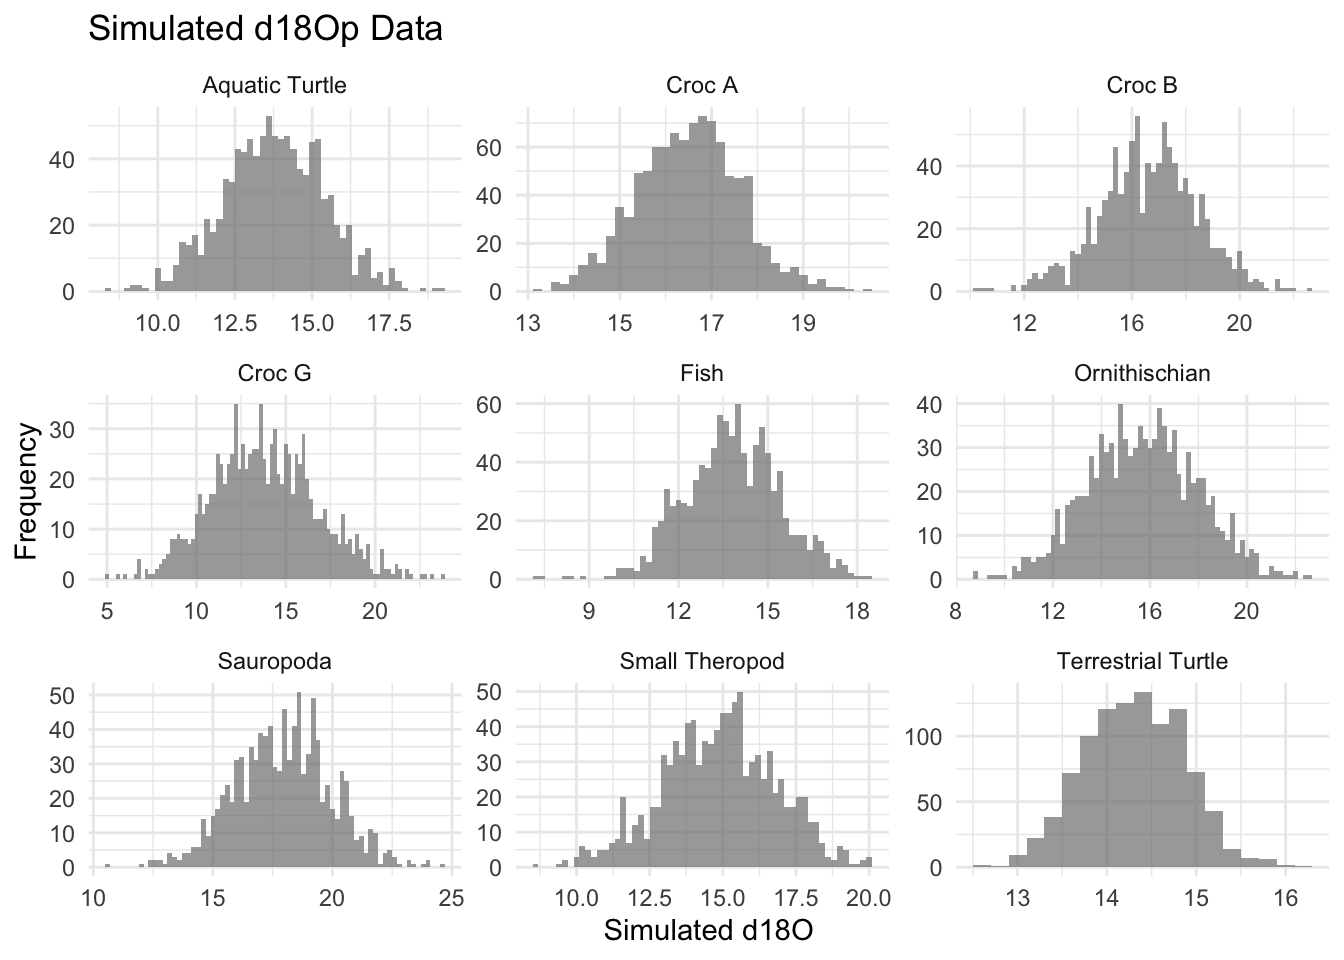
\includegraphics{V1075_MonteCarlo_files/figure-latex/unnamed-chunk-2-1.pdf}

\hypertarget{step-3-calculate-water-oxygen-isotope-values-from-simulated-turtle-samples}{%
\subsection{Step 3: Calculate water oxygen isotope values from simulated
turtle
samples}\label{step-3-calculate-water-oxygen-isotope-values-from-simulated-turtle-samples}}

Note that we are only using data from an aquatic turtle genus Glyptops
spp. It is important to choose a turtle taxon that is thought to have
been mostly or entirely aquatic in habit.

We'll do this using the relationship between environmental water and
turtle bone defined by Barrick et al.~(1999).

\begin{Shaded}
\begin{Highlighting}[]
\CommentTok{\# calculate water}

  \CommentTok{\# create function}
\NormalTok{    turtlewater }\OtherTok{\textless{}{-}} \ControlFlowTok{function}\NormalTok{(synthmeans\_turtle)\{}
      \FloatTok{1.01} \SpecialCharTok{*}\NormalTok{(synthmeans\_turtle) }\SpecialCharTok{{-}} \FloatTok{22.3} \CommentTok{\#Barrick et al. (1999)}
\NormalTok{    \}}

  \CommentTok{\# run turtlewater on synth\_turtle}
\NormalTok{    synth\_turtle }\OtherTok{\textless{}{-}}\NormalTok{ synth\_turtle }\SpecialCharTok{\%\textgreater{}\%}
      \FunctionTok{mutate}\NormalTok{(}\AttributeTok{d18Owater =} \FunctionTok{turtlewater}\NormalTok{(means))}

\CommentTok{\# Plot histogram of d18Owater}
  \FunctionTok{ggplot}\NormalTok{(synth\_turtle, }\FunctionTok{aes}\NormalTok{(}\AttributeTok{x =}\NormalTok{ d18Owater, }\AttributeTok{fill =} \StringTok{"Turtle"}\NormalTok{)) }\SpecialCharTok{+}
    \FunctionTok{geom\_histogram}\NormalTok{(}\AttributeTok{position =} \StringTok{"identity"}\NormalTok{, }\AttributeTok{alpha =} \FloatTok{0.7}\NormalTok{, }\AttributeTok{bins =} \DecValTok{30}\NormalTok{, }\AttributeTok{color =} \StringTok{"black"}\NormalTok{) }\SpecialCharTok{+}
    \FunctionTok{labs}\NormalTok{(}\AttributeTok{title =} \StringTok{"Histogram of d18Owater"}\NormalTok{,}
         \AttributeTok{x =} \StringTok{"d18Owater"}\NormalTok{,}
         \AttributeTok{y =} \StringTok{"Frequency"}\NormalTok{) }\SpecialCharTok{+}
    \FunctionTok{theme\_minimal}\NormalTok{() }\SpecialCharTok{+}
    \FunctionTok{scale\_fill\_manual}\NormalTok{(}\AttributeTok{values =} \FunctionTok{c}\NormalTok{(}\StringTok{"\#1f78b4"}\NormalTok{))}
\end{Highlighting}
\end{Shaded}

\includegraphics{V1075_MonteCarlo_files/figure-latex/unnamed-chunk-3-1.pdf}

\begin{Shaded}
\begin{Highlighting}[]
  \CommentTok{\# CI, mean of turtle d18Owater}
\NormalTok{    CIsetup\_water }\OtherTok{\textless{}{-}} \FunctionTok{sort}\NormalTok{(synth\_turtle}\SpecialCharTok{$}\NormalTok{d18Owater)}
    
    \CommentTok{\# Calculate the lower and upper percentiles for the middle 95\%}
\NormalTok{    lower\_percentile\_water }\OtherTok{\textless{}{-}} \FunctionTok{quantile}\NormalTok{(CIsetup\_water, }\FloatTok{0.025}\NormalTok{)}
\NormalTok{    upper\_percentile\_water }\OtherTok{\textless{}{-}} \FunctionTok{quantile}\NormalTok{(CIsetup\_water, }\FloatTok{0.975}\NormalTok{)}
    
    \CommentTok{\# Subset the middle 95\% of the data}
\NormalTok{    subset\_CIsetup\_water }\OtherTok{\textless{}{-}}\NormalTok{ CIsetup\_water[CIsetup\_water }\SpecialCharTok{\textgreater{}=}\NormalTok{ lower\_percentile\_water }\SpecialCharTok{\&}\NormalTok{ CIsetup\_water }\SpecialCharTok{\textless{}=}\NormalTok{ upper\_percentile\_water]}
    
    \CommentTok{\# Take mean}
\NormalTok{    mean\_turtlewater }\OtherTok{\textless{}{-}} \FunctionTok{round}\NormalTok{(}\FunctionTok{mean}\NormalTok{(subset\_CIsetup\_water), }\DecValTok{1}\NormalTok{)}
\NormalTok{    lowCI\_water }\OtherTok{\textless{}{-}} \FunctionTok{round}\NormalTok{(}\FunctionTok{abs}\NormalTok{(mean\_turtlewater }\SpecialCharTok{{-}}\NormalTok{ lower\_percentile\_water), }\DecValTok{1}\NormalTok{)}
\NormalTok{    highCI\_water }\OtherTok{\textless{}{-}} \FunctionTok{round}\NormalTok{(}\FunctionTok{abs}\NormalTok{(mean\_turtlewater }\SpecialCharTok{{-}}\NormalTok{ upper\_percentile\_water), }\DecValTok{1}\NormalTok{)}
    \FunctionTok{cat}\NormalTok{(mean\_turtlewater, }\StringTok{"+"}\NormalTok{, highCI\_water, }\StringTok{"/"}\NormalTok{, }\StringTok{"{-}"}\NormalTok{, lowCI\_water)}
\end{Highlighting}
\end{Shaded}

\begin{verbatim}
## -8 + 0.6 / - 0.6
\end{verbatim}

\hypertarget{step-4-calculate-temperatures}{%
\subsection{Step 4: Calculate
temperatures}\label{step-4-calculate-temperatures}}

We'll use the relationship between
\(\delta\)\textsuperscript{18}O\textsubscript{phosphate} and temperature
defined originally by Longinelli \& Nuti (1973) and refined by
Puc\textquotesingle eat et al.~(2010)

\begin{Shaded}
\begin{Highlighting}[]
\CommentTok{\# calculate temps}
    \CommentTok{\# define temp function}
\NormalTok{    TempFun }\OtherTok{\textless{}{-}} \ControlFlowTok{function}\NormalTok{(d18Ofish, NISTmean, d18Owater) \{}
\NormalTok{      temp }\OtherTok{\textless{}{-}} \FloatTok{118.7} \SpecialCharTok{{-}} \FloatTok{4.22}\SpecialCharTok{*}\NormalTok{((d18Ofish  }\SpecialCharTok{+}\NormalTok{(}\FloatTok{22.6} \SpecialCharTok{{-}}\NormalTok{ NISTmean)) }\SpecialCharTok{{-}}\NormalTok{ d18Owater) }
\NormalTok{    \}}

    \CommentTok{\# run TempFun over all the synthetic means}
\NormalTok{    synth\_temps }\OtherTok{\textless{}{-}} \FunctionTok{TempFun}\NormalTok{(}\AttributeTok{d18Ofish =}\NormalTok{ synth\_gar}\SpecialCharTok{$}\NormalTok{means, }
                           \AttributeTok{NISTmean =}\NormalTok{ synth\_NIST}\SpecialCharTok{$}\NormalTok{means,}
                           \AttributeTok{d18Owater =}\NormalTok{ synth\_turtle}\SpecialCharTok{$}\NormalTok{d18Owater)}
    
\CommentTok{\# Plot the temperatures}
  \FunctionTok{ggplot}\NormalTok{(}\AttributeTok{data =} \FunctionTok{data.frame}\NormalTok{(}\AttributeTok{temperature =}\NormalTok{ synth\_temps), }\FunctionTok{aes}\NormalTok{(}\AttributeTok{x =}\NormalTok{ temperature)) }\SpecialCharTok{+}
        \FunctionTok{geom\_histogram}\NormalTok{(}\AttributeTok{binwidth =} \DecValTok{1}\NormalTok{, }\AttributeTok{fill =} \FunctionTok{c}\NormalTok{(}\StringTok{"\#ff0000"}\NormalTok{), }\AttributeTok{color =} \StringTok{"black"}\NormalTok{, }\AttributeTok{alpha =} \FloatTok{0.7}\NormalTok{) }\SpecialCharTok{+}
        \FunctionTok{labs}\NormalTok{(}\AttributeTok{title =} \StringTok{"Histogram of Temperatures"}\NormalTok{,}
             \AttributeTok{x =} \StringTok{"Temperature (degrees C)"}\NormalTok{,}
             \AttributeTok{y =} \StringTok{"Frequency"}\NormalTok{)}
\end{Highlighting}
\end{Shaded}

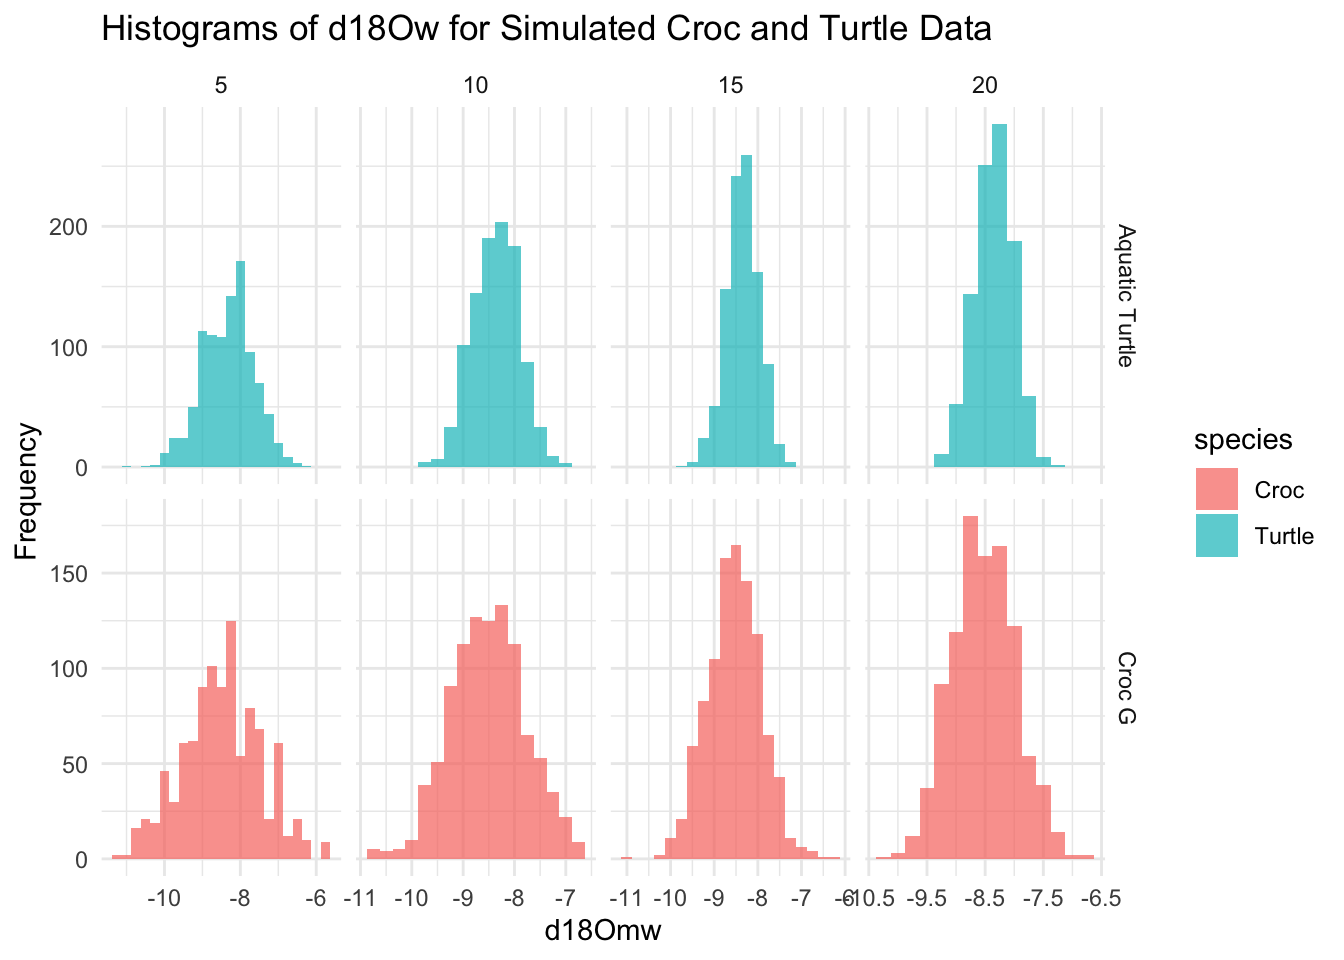
\includegraphics{V1075_MonteCarlo_files/figure-latex/unnamed-chunk-4-1.pdf}

\hypertarget{step-5-confidence-intervals}
\NormalTok{    lower\_percentile }\OtherTok{\textless{}{-}} \FunctionTok{quantile}\NormalTok{(CIsetup, }\FloatTok{0.025}\NormalTok{)}
\NormalTok{    upper\_percentile }\OtherTok{\textless{}{-}} \FunctionTok{quantile}\NormalTok{(CIsetup, }\FloatTok{0.975}\NormalTok{)}
    
\CommentTok{\# Subset the middle 95\% of the data}
\NormalTok{    subset\_CIsetup }\OtherTok{\textless{}{-}}\NormalTok{ CIsetup[CIsetup }\SpecialCharTok{\textgreater{}=}\NormalTok{ lower\_percentile }\SpecialCharTok{\&}\NormalTok{ CIsetup }\SpecialCharTok{\textless{}=}\NormalTok{ upper\_percentile]}
    
\CommentTok{\# Take mean}
\NormalTok{    mean\_temp }\OtherTok{\textless{}{-}} \FunctionTok{round}\NormalTok{(}\FunctionTok{mean}\NormalTok{(subset\_CIsetup), }\DecValTok{1}\NormalTok{)}
\NormalTok{    lowCI }\OtherTok{\textless{}{-}} \FunctionTok{round}\NormalTok{(}\FunctionTok{abs}\NormalTok{(mean\_temp }\SpecialCharTok{{-}}\NormalTok{ lower\_percentile), }\DecValTok{1}\NormalTok{)}
\NormalTok{    highCI }\OtherTok{\textless{}{-}} \FunctionTok{round}\NormalTok{(}\FunctionTok{abs}\NormalTok{(mean\_temp }\SpecialCharTok{{-}}\NormalTok{ upper\_percentile), }\DecValTok{1}\NormalTok{)}
    \FunctionTok{cat}\NormalTok{(mean\_temp, }\StringTok{"+"}\NormalTok{, highCI, }\StringTok{"/"}\NormalTok{, }\StringTok{"{-}"}\NormalTok{, lowCI)}
\end{Highlighting}
\end{Shaded}

\begin{verbatim}
## 25 + 3.7 / - 3.7
\end{verbatim}

\end{document}
